\documentclass[14pt]{beamer}

\usepackage[british]{babel}

\usepackage{graphicx}
\usepackage{amssymb}
\usepackage{color}
\usepackage{listings}
\usepackage{xspace}

\newcommand{\splang}{\textsc{Splang}\xspace}

\title{\splang}
\author{Wouter Geraedts \and Joshua Moerman}
\institute{Radboud Universiteit Nijmegen}
\date{}

\begin{document}

\begin{frame}
\titlepage
\end{frame}


\begin{frame}
\frametitle{\splang}
\splang is implemented in Haskell
\bigskip

Pros:
\begin{itemize}
	\item Ease of implementing AST
	\item Do-syntax for monads
\end{itemize}

Cons:
\begin{itemize}
	\item No generics as in Clean
\end{itemize}
\end{frame}


\begin{frame}
We made our own parser combinators (non-deterministic).
\begin{itemize}
	\item Propagates source-information
	\item Nice error messages (see demo)
\end{itemize}

Scanner skips the whitespace and comments and recognizes keywords, number and identifiers.

Changes in parser consist of prioritizing operators.
\end{frame}


\begin{frame}
We used \texttt{ansi-terminal} and \texttt{edit-distance} for colors and suggestions (see demo).

We spent quite some time to make \splang your best friend :). (Aka $x$ hours.)
\end{frame}


\begin{frame}
\frametitle{Ambiguity + Pretty Printing}
\begin{center}
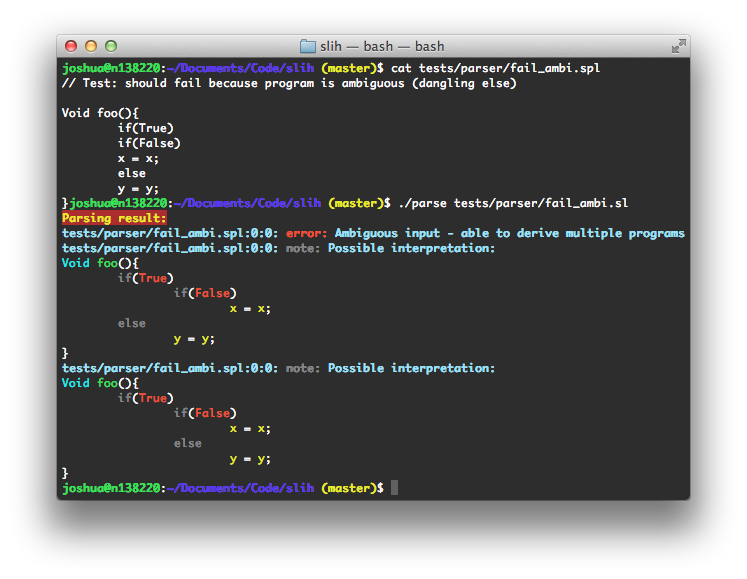
\includegraphics[width=\textwidth]{ambi_pretty.png}
\end{center}
\end{frame}


\begin{frame}
\frametitle{Next Phase (stub)}
\begin{center}
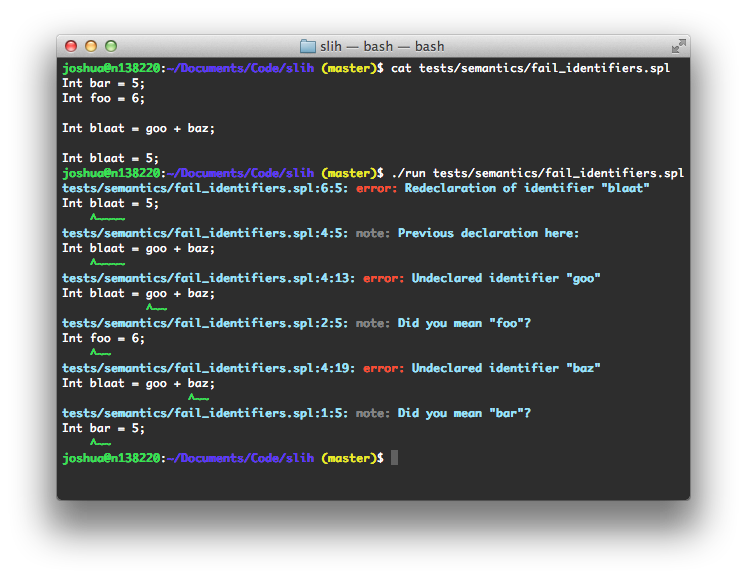
\includegraphics[width=\textwidth]{next_phase.png}
\end{center}
\end{frame}


\begin{frame}
\begin{center}
\Huge Questions?
\end{center}
\end{frame}

\end{document}
